\documentclass[tikz,border=1cm]{standalone}
\usepackage[dvipsnames]{xcolor}
\begin{document}

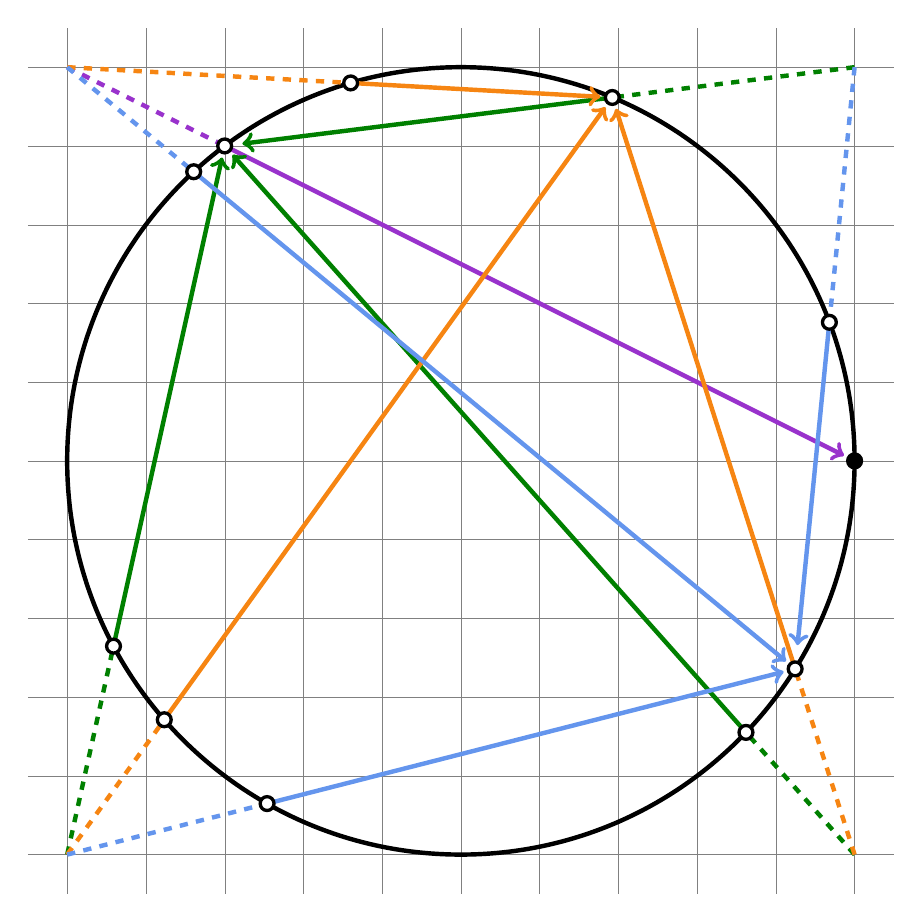
\begin{tikzpicture}[scale=5]
  \draw[gray,ultra thin] (-1.1,-1.1) grid[step=0.2] (1.1,1.1);
  \draw[ultra thick] (0,0) circle (1);
  \coordinate (Q1) at ({-3/5},{4/5});
  \coordinate (Q2) at ({5/13},{12/13});
  \coordinate (Q3) at ({21/29},{-20/29});
  \coordinate (Q4) at ({-15/17},{-8/17});
  \coordinate (Q5) at ({-7/25},{24/25});
  \coordinate (Q6) at ({-55/73},{-48/73});
  \coordinate (Q7) at ({45/53},{-28/53});
  \coordinate (P1) at ({117/125},{44/125});
  \coordinate (P2) at ({-95/193},{-168/193});
  \coordinate (P3) at ({-207/305},{224/305});

  \draw[DarkOrchid,ultra thick,dashed] (-1,1) -- (Q1);
  \draw[DarkOrchid,ultra thick,->,shorten >=1ex] (Q1) -- (1,0);
  \draw[Green,ultra thick,dashed] (1,1) -- (Q2);
  \draw[Green,ultra thick,->,shorten >=1.5ex] (Q2) -- (Q1);
  \draw[Green,ultra thick,dashed] (-1,-1) -- (Q4);
  \draw[Green,ultra thick,->,shorten >=1ex] (Q4) -- (Q1);
  \draw[Green,ultra thick,dashed] (1,-1) -- (Q3);
  \draw[Green,ultra thick,->,shorten >=1ex] (Q3) -- (Q1);
  \draw[BurntOrange,ultra thick,dashed] (-1,1) -- (Q5);
  \draw[BurntOrange,ultra thick,->,shorten >=1ex] (Q5) -- (Q2);
  \draw[BurntOrange,ultra thick,dashed] (-1,-1) -- (Q6);
  \draw[BurntOrange,ultra thick,->,shorten >=1ex] (Q6) -- (Q2);
  \draw[BurntOrange,ultra thick,dashed] (1,-1) -- (Q7);
  \draw[BurntOrange,ultra thick,->,shorten >=1ex] (Q7) -- (Q2);
  \draw[CornflowerBlue,ultra thick,dashed] (1,1) -- (P1);
  \draw[CornflowerBlue,ultra thick,dashed] (-1,1) -- (P3);
  \draw[CornflowerBlue,ultra thick,dashed] (-1,-1) -- (P2);
  \draw[CornflowerBlue,ultra thick,->,shorten >=2ex] (P1) -- (Q7);
  \draw[CornflowerBlue,ultra thick,->,shorten >=1ex] (P3) -- (Q7);
  \draw[CornflowerBlue,ultra thick,->,shorten >=1ex] (P2) -- (Q7);
  
  \draw[fill=white,very thick] (Q1) circle (.5pt);
  \draw[fill=white,very thick] (Q2) circle (.5pt);
  \draw[fill=white,very thick] (Q3) circle (.5pt);
  \draw[fill=white,very thick] (Q4) circle (.5pt);
  \draw[fill=white,very thick] (Q5) circle (.5pt);
  \draw[fill=white,very thick] (Q6) circle (.5pt);
  \draw[fill=white,very thick] (Q7) circle (.5pt);      
  \draw[fill=white,very thick] (P1) circle (.5pt);
  \draw[fill=white,very thick] (P2) circle (.5pt);
  \draw[fill=white,very thick] (P3) circle (.5pt);
  \draw[fill=black,very thick] (1,0) circle (.5pt);
\end{tikzpicture}

\end{document}
